\documentclass[12pt]{article}
\usepackage[utf8]{inputenc}
\usepackage[spanish]{babel}
\usepackage{graphicx}
\usepackage{vmargin}
\setpapersize{A4}
\setmargins{2.5cm}
{1.5cm}
{15cm}
{23.42cm}
{10pt}
{1cm}
{0pt}
{2cm}
\begin{document}	

\begin{titlepage}
     \begin{center}
     \bigskip
    
    \textbf{Universidad Nacional Autónoma de México}
    
    \bigskip
    \bigskip
    
    Facultad de Ciencias
    
    \bigskip
    \bigskip
    
    

\begin{figure}[htb]
	\centering
	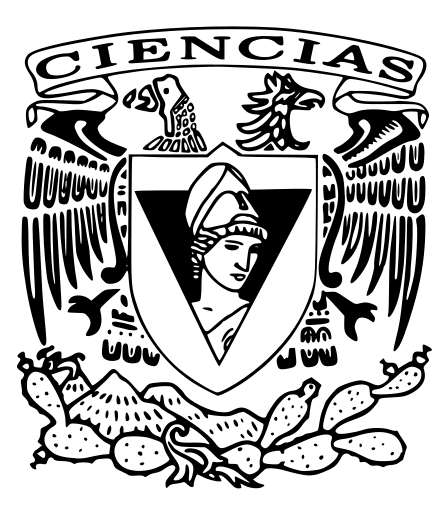
\includegraphics[width=5cm]{ciencias.png}
	\label{fig:ejemplo1}
\end{figure}



    
    
    \begin{Large}
    
      Descripción de las ecuaciones básicas de la electrostática y semblanza de los premios Nobel de los años 2017,2018 y 2019
      
    \end{Large} 
   
    \rule{100mm}{0.5mm}
   
    \bigskip
    \bigskip
   
   Héctor Jair Morales Gómez 
   
   \bigskip
   \bigskip
   
    \textbf{Tarea 2}

    \bigskip
    Computación
\end{center}
\end{titlepage}


\section{Introducción}

Lorem ipsum dolor sit amet, consectetur adipiscing elit. Praesent non sapien eget eros iaculis porttitor sit amet id risus. Donec rhoncus consequat mauris, sit amet varius sem hendrerit ac. In hac habitasse platea dictumst. Curabitur iaculis eros eget justo efficitur, vitae consequat neque posuere. Nunc vitae viverra orci. Cras eget lorem sit amet massa sagittis placerat. Vestibulum lobortis quis lectus sit amet tristique. Sed nec volutpat justo, ac placerat dui. 


\section{Desarrollo}

Lorem ipsum dolor sit amet, consectetur adipiscing elit. Praesent non sapien eget eros iaculis porttitor sit amet id risus. Donec rhoncus consequat mauris, sit amet varius sem hendrerit ac. In hac habitasse platea dictumst. Curabitur iaculis eros eget justo efficitur, vitae consequat neque posuere. Nunc vitae viverra orci. Cras eget lorem sit amet massa sagittis placerat. Vestibulum lobortis quis lectus sit amet tristique. Sed nec volutpat justo, ac placerat dui. 

\subsubsection{Leyes de Maxwell}

Lorem ipsum dolor sit amet, consectetur adipiscing elit. Praesent non sapien eget eros iaculis porttitor sit amet id risus. Donec rhoncus consequat mauris, sit amet varius sem hendrerit ac. In hac habitasse platea dictumst.

\begin{equation}
    \vec{\nabla} \cdot \vec{E}=\frac{\rho}{\varepsilon_{0}}
\end{equation}
\begin{equation}
    \vec{\nabla} \cdot \vec{B}=0
\end{equation}
\begin{equation}
    \vec{\nabla} \times \vec{E}=-\frac{\partial \vec{B}}{\partial t}
\end{equation}
\begin{equation}
    \vec{\nabla} \times \vec{B}=\mu_{0} \vec{J}+\mu_{0} \varepsilon_{0} \frac{\partial \vec{E}}{\partial t}
\end{equation}

Lorem ipsum dolor sit amet, consectetur adipiscing elit. Praesent non sapien eget eros iaculis porttitor sit amet id risus. Donec rhoncus consequat mauris, sit amet varius sem hendrerit ac. In hac habitasse platea dictumst.

\begin{equation}
    \oint_{S} \vec{E} \cdot \mathrm{d} \vec{S}=\frac{q}{\varepsilon_{0}}
\end{equation}
\begin{equation}
    \oint_{s} \vec{B} \cdot \mathrm{d} \vec{S}=0
\end{equation}
\begin{equation}
    \oint \vec{E} \cdot \mathrm{d} \vec{\ell}=-\int_{S} \frac{\mathrm{d} \vec{B}}{\mathrm{d} t} \cdot \mathrm{d} \vec{S}
\end{equation}
\begin{equation}
    \oint_{C} \vec{B} \cdot \mathrm{d} \vec{\ell}=\mu_{0} \int_{S} \vec{J} \cdot \mathrm{d} \vec{S}+\mu_{0} \varepsilon_{0} \frac{\mathrm{d}}{\mathrm{d} t} \int_{S} \vec{E} \cdot \mathrm{d} \vec{S}
\end{equation}

\subsubsection{Ecuaciones básicas de la electrostática}

Pellentesque nec suscipit arcu. Duis ac viverra justo. Morbi accumsan magna justo, vitae auctor massa feugiat vulputate. Integer maximus felis eget turpis consectetur, non aliquet lectus condimentum. Morbi interdum volutpat urna ac tristique. Nam a ante congue, laoreet leo nec, dictum quam. Fusce in ipsum in odio semper interdum. 

\begin{equation}
    |\boldsymbol{F}|=k_{e} \frac{\left|q_{1} q_{2}\right|}{r^{2}}
\end{equation}
\begin{equation}
    \boldsymbol{F}_{1}=\frac{q_{1} q_{2}}{4 \pi \varepsilon_{0}} \frac{\left(\boldsymbol{r}_{1}-\boldsymbol{r}_{2}\right)}{\left|\boldsymbol{r}_{1}-\boldsymbol{r}_{2}\right|^{3}}=\frac{q_{1} q_{2}}{4 \pi \varepsilon_{0}} \frac{\widehat{\boldsymbol{r}}_{21}}{\left|\boldsymbol{r}_{21}\right|^{2}}
\end{equation}

\medskip

Pellentesque nec suscipit arcu. Duis ac viverra justo. Morbi accumsan magna justo, vitae auctor massa feugiat vulputate. Integer maximus felis eget turpis consectetur, non aliquet lectus condimentum. Morbi interdum volutpat urna ac tristique. Nam a ante congue, laoreet leo nec, dictum quam. Fusce in ipsum in odio semper interdum. 

\begin{equation}
    \boldsymbol{F}(\boldsymbol{r})=\frac{q}{4 \pi \varepsilon_{0}} \sum_{i=1}^{N} q_{i} \frac{\boldsymbol{r}-\boldsymbol{r}_{i}}{\left|\boldsymbol{r}-\boldsymbol{r}_{i}\right|^{3}}=\frac{q}{4 \pi \varepsilon_{0}} \sum_{i=1}^{N} q_{i} \frac{\widehat{\boldsymbol{R}}_{i}}{\left|\boldsymbol{R}_{i}\right|^{2}}
\end{equation}

Pellentesque nec suscipit arcu. Duis ac viverra justo. Morbi accumsan magna justo, vitae auctor massa feugiat vulputate. Integer maximus felis eget turpis consectetur, non aliquet lectus condimentum. Morbi interdum volutpat urna ac tristique. Nam a ante congue, laoreet leo nec, dictum quam. Fusce in ipsum in odio semper interdum [1]. 

\medskip

\begin{equation}
    \mathbf{F}=q \mathbf{E}
\end{equation}
\begin{equation}
    \boldsymbol{F}=\frac{1}{4 \pi \varepsilon_{0}} \frac{q_{1} q_{0}}{\left(\boldsymbol{x}_{1}-\boldsymbol{x}_{0}\right)^{2}} \hat{\boldsymbol{r}}_{1,0}
\end{equation}

\medskip

\subsection{Semblanza de los últimos premios Nobel}

Vestibulum consectetur ac est nec condimentum. Integer convallis, arcu quis lacinia consectetur, ligula nisi congue sapien, quis tempor nulla velit feugiat nisl. Curabitur fringilla, felis volutpat imperdiet eleifend, libero nibh semper erat, eget vehicula dolor lectus in nunc. Vestibulum consequat leo arcu, vitae convallis metus finibus ac. Maecenas fermentum velit finibus purus sagittis posuere vitae ut est. Quisque mauris nunc, tincidunt a sem laoreet, cursus mattis enim. Vestibulum ante ipsum primis in faucibus orci luctus et ultrices posuere cubilia Curae; Sed id nunc eget lorem cursus suscipit non vel ligula. Donec nec dolor metus. Nulla tempus purus nec ullamcorper congue. Etiam consequat nulla nulla, bibendum porta nisi pulvinar sed. Nullam ultrices lacinia bibendum. Vestibulum sed mauris vitae justo convallis ullamcorper.

\bigskip

\subsubsection{Premio Nobel en física del 2016}

Lorem ipsum dolor sit amet, consectetur adipiscing elit. Praesent non sapien eget eros iaculis porttitor sit amet id risus. Donec rhoncus consequat mauris, sit amet varius sem hendrerit ac. In hac habitasse platea dictumst. Curabitur iaculis eros eget justo efficitur, vitae consequat neque posuere. Nunc vitae viverra orci. Cras eget lorem sit amet massa sagittis placerat. Vestibulum lobortis quis lectus sit amet tristique. Sed nec volutpat justo, ac placerat dui[2]. 

\subsubsection{Premio Nobel en física del 2017}

Lorem ipsum dolor sit amet, consectetur adipiscing elit. Praesent non sapien eget eros iaculis porttitor sit amet id risus. Donec rhoncus consequat mauris, sit amet varius sem hendrerit ac. In hac habitasse platea dictumst. Curabitur iaculis eros eget justo efficitur, vitae consequat neque posuere. Nunc vitae viverra orci. Cras eget lorem sit amet massa sagittis placerat. Vestibulum lobortis quis lectus sit amet tristique. Sed nec volutpat justo, ac placerat dui[3]. 

\subsubsection{Premio Nobel en física del 2018}

Lorem ipsum dolor sit amet, consectetur adipiscing elit. Praesent non sapien eget eros iaculis porttitor sit amet id risus. Donec rhoncus consequat mauris, sit amet varius sem hendrerit ac. In hac habitasse platea dictumst. Curabitur iaculis eros eget justo efficitur, vitae consequat neque posuere. Nunc vitae viverra orci. Cras eget lorem sit amet massa sagittis placerat. Vestibulum lobortis quis lectus sit amet tristique. Sed nec volutpat justo, ac placerat dui[4]. 

\begin{thebibliography}{999}

\bibitem{[1]}
 Peskin, M. E. (2018). An introduction to quantum field theory. CRC Press.
  
\bibitem{[2]}
 Itzykson, C., & Zuber, J. B. (2012). Quantum field theory. Courier Corporation.
  
\bibitem{[3]}
 Kaku, M. (1993). Quantum field theory: a modern introduction. Oxford Univ. Press.
 
 \bibitem{[4]}
 Peskin, M. E. (2018). An introduction to quantum field theory. CRC Press.
  
\bibitem{[5]}
 Itzykson, C., & Zuber, J. B. (2012). Quantum field theory. Courier Corporation.
  
\bibitem{[6]}
 Kaku, M. (1993). Quantum field theory: a modern introduction. Oxford Univ. Press.
 
 \bibitem{[7]}
 Kaku, M. (1993). Quantum field theory: a modern introduction. Oxford Univ. Press.
 

\end{thebibliography}



\end{document}